\subsection{Front-end}

As mentioned in the requirements, I used React for the front-end. The main folder structure can be seen in the appendices \hyperref[front-end-tree]{front-end-tree}. I used \textbf{antd}, an enterprise-class UI design language and React UI library, for the user interface, Node.js, a JavaScript runtime built on Chrome's V8 JavaScript engine, and npm, packages manager.

The front-end part has two main folders: public and src. The folder `public' contains the default \texttt{public.html} when npm is used to create the project, and \texttt{public.html} contains only one div whose id is `\texttt{root}' and which will be modified through entire app. 

\subsubsection{Folder Structure}

The main project files are inside the src folder.
\begin{itemize}
  \item \texttt{globals}: It is a folder containing the app's global variables.
  \item \texttt{pages}: It is a folder containing the pages called auth, book, and user, as well as the main homepage of the app.
  \item \texttt{service}: It is a folder containing the front-end service layer. Files inside this folder include functions to connect the back-end.
  \item \texttt{App.js}: It is a file and is responsible for rendering the pages and providing the main/top navigations around the app. Also, it checks the authorization token and its validation.
  \item \texttt{index.js}: It is a file and responsible for rendering \texttt{App.js} by using \texttt{ReactDOM}.
\end{itemize}

I will briefly explain the folder and files in detail. Then I will tell the pages.

\paragraph{\texttt{globals}}

This folder contains just a file called \texttt{GlobalVariables}. That file includes two global variables, called \texttt{BOOK\_COLUMNS} and \texttt{PAGINATION}, which are used for tables around the app.

\begin{figure}[ht]
  \centering
  \begin{forest}
    pic dir tree,
    where level=0{}{% folder icons by default; override using file for file icons
      directory,
    },
    [\dots
      [globals
        [GlobalVariables.js, file]
      ]
    ]
  \end{forest}
  \caption{Structue of globals}
\end{figure}

\paragraph{\texttt{pages}} 

This folder contains the whole pages, which means users mainly see the files inside this folder. I will explain the pages in detail later.

\begin{figure}[ht]
  \centering
  \begin{forest}
    pic dir tree,
    where level=0{}{% folder icons by default; override using file for file icons
      directory,
    },
    [\dots
      [pages
        [auth
          [\dots, file]
        ]
        [book
          [\dots]
        ]
        [user
          [\dots]
        ]
        [Home.js, file]
      ]
    ]
  \end{forest}
  \caption{Structue of pages}
\end{figure}

\begin{itemize}
  \item \texttt{Home.js}: This is the app's homepage and contains the user's general information. It can be accessed by clicking the \texttt{Home} from the top navigation.
  
  \item \texttt{auth}: This folder contains just a file called \texttt{Login}, which is responsible for the login page.
  
  \item \texttt{book}: This is the page of books. It contains five folders and one file inside it and is responsible for the operations of adding, deleting, updating, and adding/removing books to/from favorite/read lists. It uses a switch for rendering the right page of the operation.
  
  \item \texttt{user}: This is the page of users. It contains four folders and one file inside it and is responsible for adding, deleting, and updating operations. It uses a switch for rendering the right page of the operation.
\end{itemize}
  
\paragraph{\texttt{service}} 

This folder contains the services to access the back-end. The functions inside the service files handle the returned response and return a new object with the data inside the response. Additionally, thanks to Axios interceptor, the authorization token, which is saved to \texttt{Session Storage} or \texttt{Local Storage} while logging in, is added to the header of all requests.

\begin{figure}[ht]
  \centering
  \begin{forest}
    pic dir tree,
    where level=0{}{% folder icons by default; override using file for file icons
      directory,
    },
    [\dots
      [service
        [AuthService.js, file]
        [BookListService.js, file]
        [BookService.js, file]
        [UserService.js, file]
      ]
    ]
  \end{forest}
  \caption{Structue of service}
\end{figure}

\begin{itemize}
  \item \texttt{AuthService}: Responsible for authentication and login process.
  \item \texttt{BookListService}: Responsible for adding/removing books to/from read/favorite lists.
  \item \texttt{BookService}: Responsible for book operations such as searching, adding, removing, and updating.
  \item \texttt{UserService}: Responsible for user operations such as searching, adding, removing, and updating.
\end{itemize}

\subsubsection{Pages}

When the app is run, firstly \texttt{index.js} renders the \texttt{App.js}. \texttt{App.js} firstly checks the authorization token and its validation. If the token is valid, it directs the user to the homepage, rendering (\texttt{Home.js}). If the token is not valid, it directs the user to the login page, rendering (\texttt{Login.js}).

\paragraph{\texttt{Login and Logout}}

This page contains a basic login form. While the login page is done by antd form, the logout item is constructed by `Popconfirm' of antd. If the `\texttt{Remember me}' option is chosen, authorization token is saved into both \texttt{Session Storage} and \texttt{Local Storage}. However, if it is not chosen, the token is only saved into \texttt{Session Storage}.

\begin{minipage}{.49\textwidth}
  \begin{figure}[H]
    \centering
  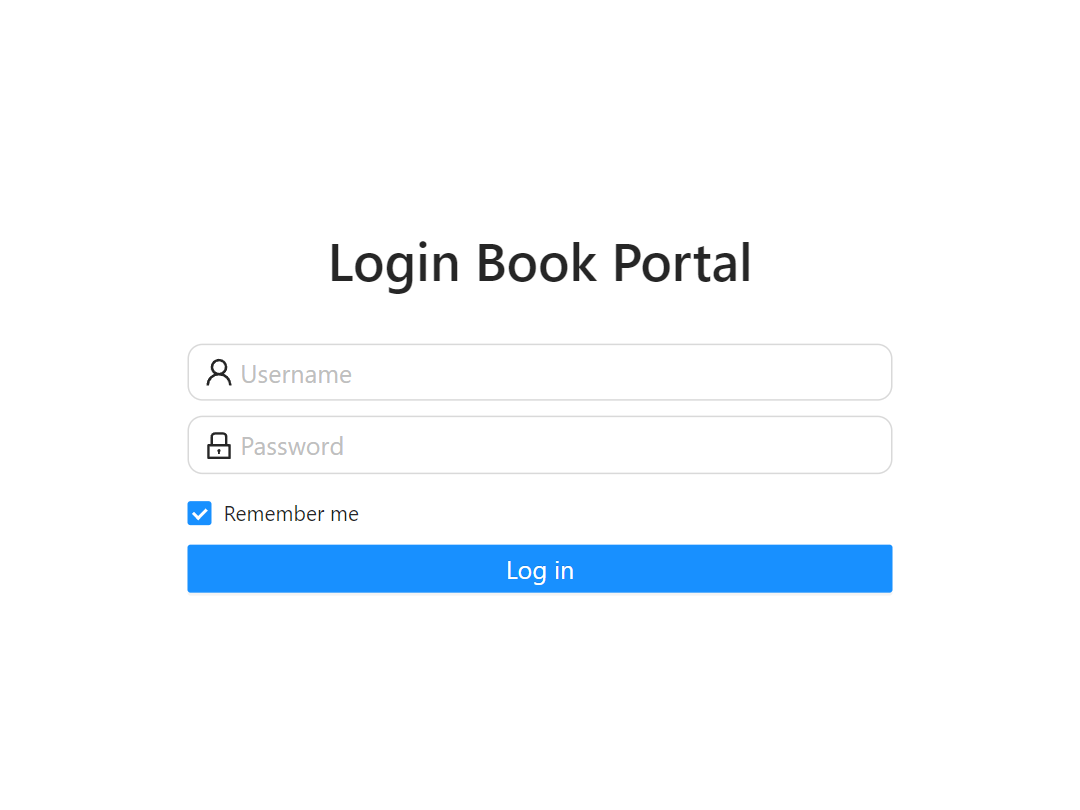
\includegraphics[width=\textwidth]{img/front-end/login-page.png}
  \caption{Login Page}
  \end{figure}
\end{minipage}
\begin{minipage}{.49\textwidth}
  \begin{figure}[H]
    \centering
  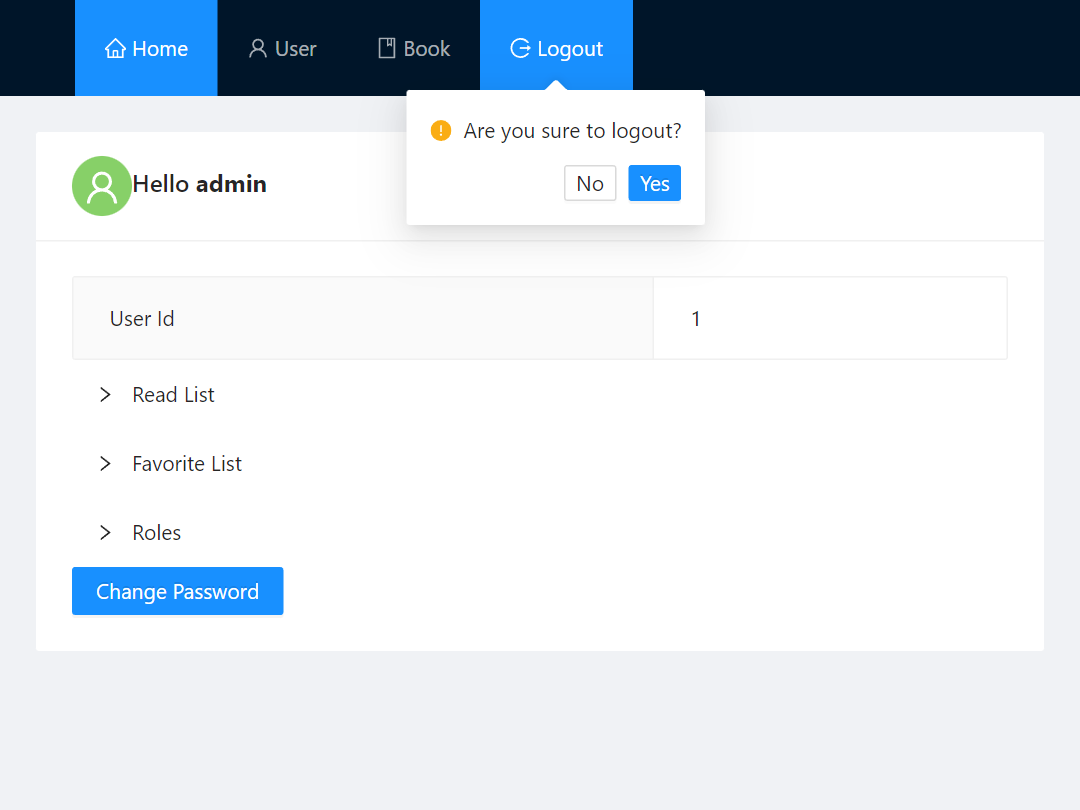
\includegraphics[width=\textwidth]{img/front-end/logout.png}
  \caption{Logout}
  \end{figure}
\end{minipage}

After logging in, users are directed to the homepage. At the top of the screen, there are four different menu items, called \texttt{Home}, \texttt{User}, \texttt{Book} and \texttt{Logout}. Home is firstly rendered, and using these navigations page can be changed.

When users click to \texttt{Logout}, a warning, which asks whether they are sure to log out, pops up. If yes is clicked, users are directed to the login page.

\paragraph{\texttt{Home}}

On the homepage, user information is provided. This page makes use of `Card', `Descriptions', `Collapse', and `Panel' of antd to show the information. Users can see their user ids, read lists, favorite lists, and roles on this screen. This information is acquired by sending back-end a request by username and setting the information state. By using the button ``Change Password'', they can also access the update form and change their passwords.

\begin{minipage}{.49\textwidth}  
  \begin{figure}[H]
    \centering
    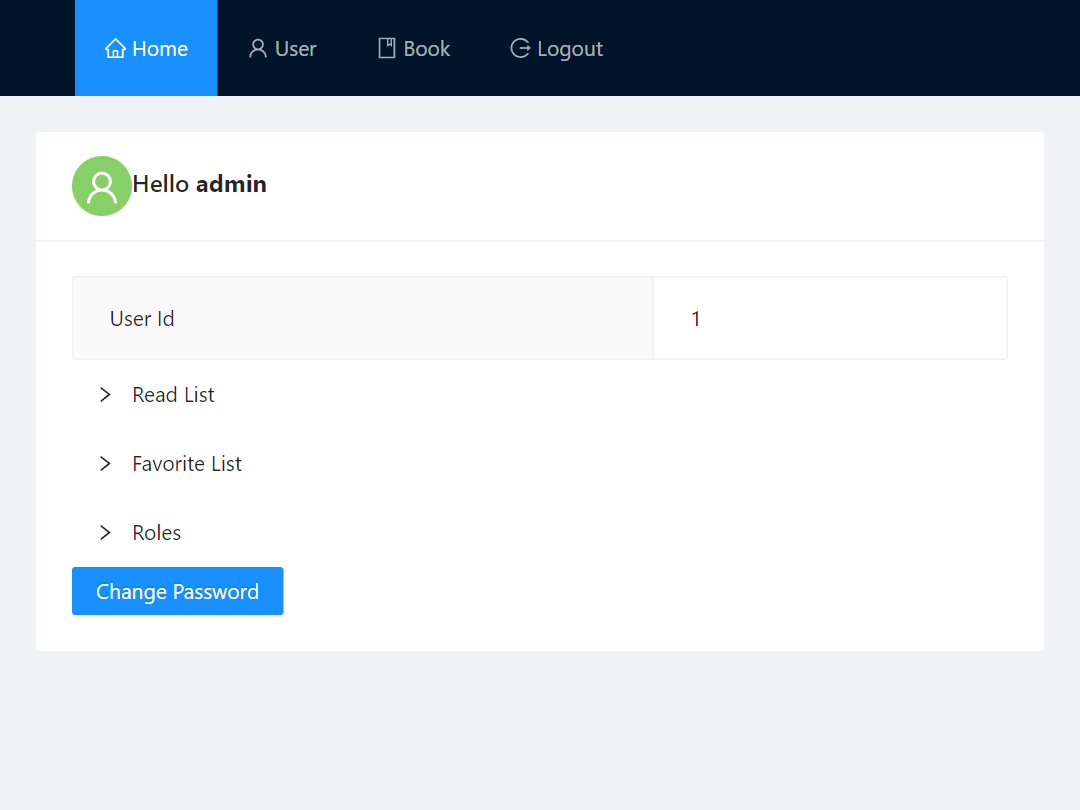
\includegraphics[width=\linewidth]{img/front-end/homepage.png}
    \caption{Home Page}
  \end{figure}
\end{minipage}
\begin{minipage}{.49\textwidth}
  \begin{figure}[H]
    \centering
    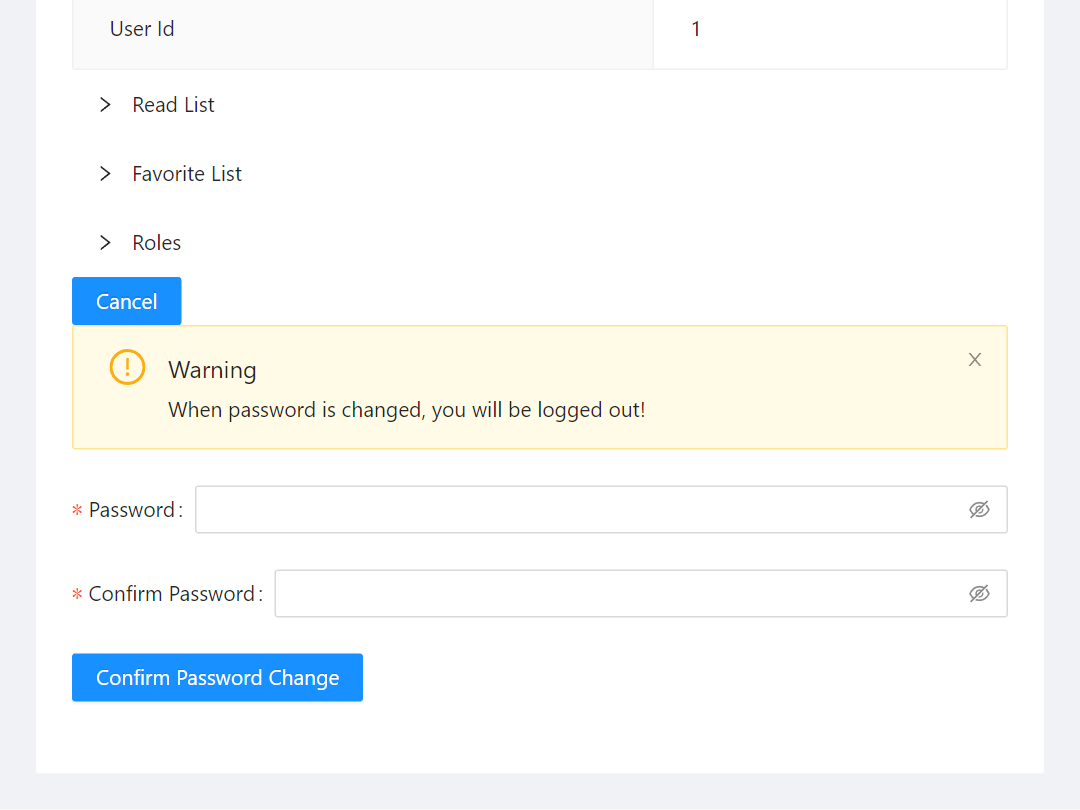
\includegraphics[width=\textwidth]{img/front-end/homepage-password.png}
    \caption{Password Change}
  \end{figure}
\end{minipage}

Since regular users are not allowed to do user operations such as adding, deleting, or updating, \texttt{User} page is unique to admins. Therefore, \texttt{User} item is not seen when the user does not have admin roles.

\begin{figure}[H]
  \centering
  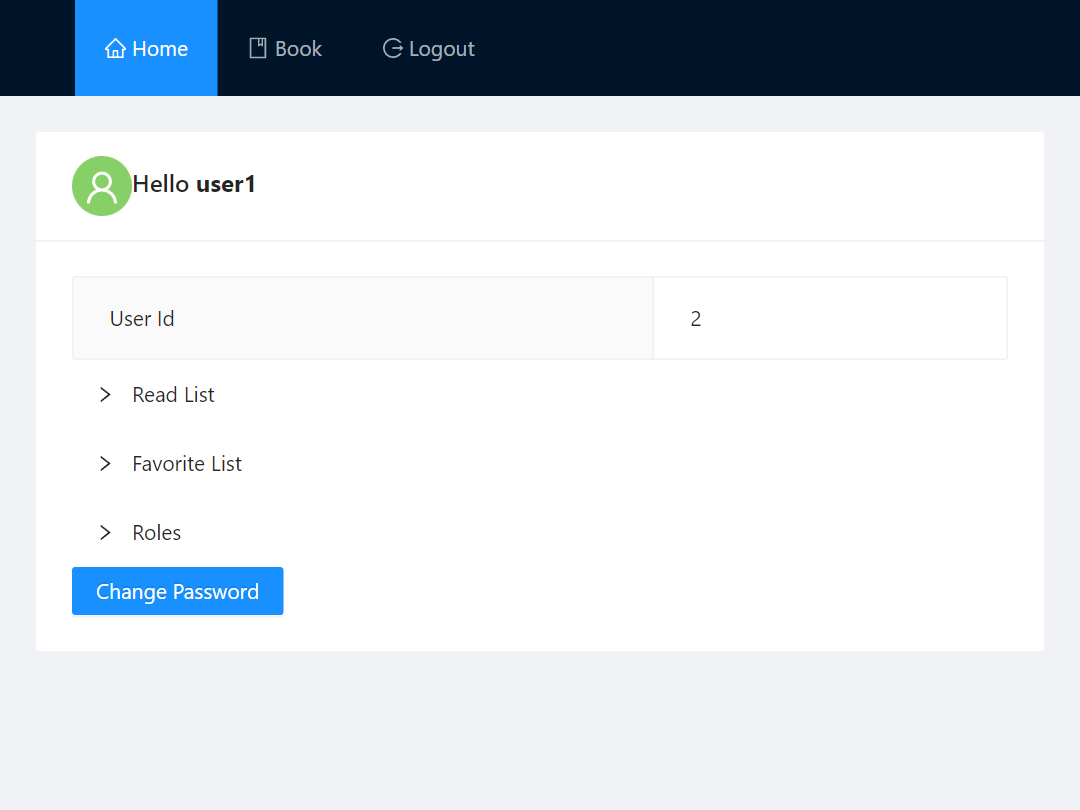
\includegraphics[width=\textwidth]{img/front-end/homepage-user.png}
  \caption{User Home Page}
\end{figure}


\paragraph{\texttt{User}}

When \texttt{User} is clicked from top navigation, \texttt{User} page is rendered. On this page, there are three operations: adding, deleting, and updating users. This page is special to admins because users are not allowed to add, delete, or update users. Therefore, this page is only accessible when the user does not have the admin role.

\begin{figure}[H]
  \centering
  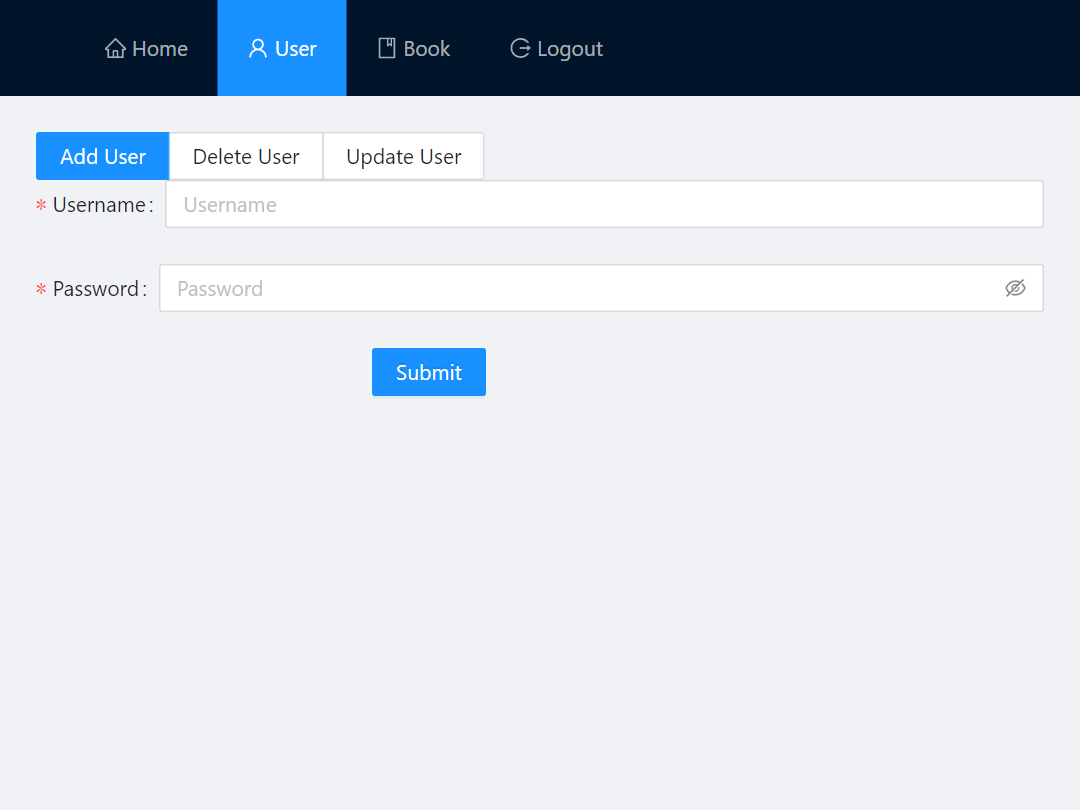
\includegraphics[width=\textwidth]{img/front-end/user.png}
  \caption{User Page}
\end{figure}

\subparagraph{$\blacksquare$ \texttt{Add User}}

By default \texttt{Add User} is rendered when \texttt{User} menu item is clicked. This page is for adding a user to the database and is unique to admins. When the page is rendered, an antd form, which includes username and password, appears.

\begin{figure}[H]
  \centering
  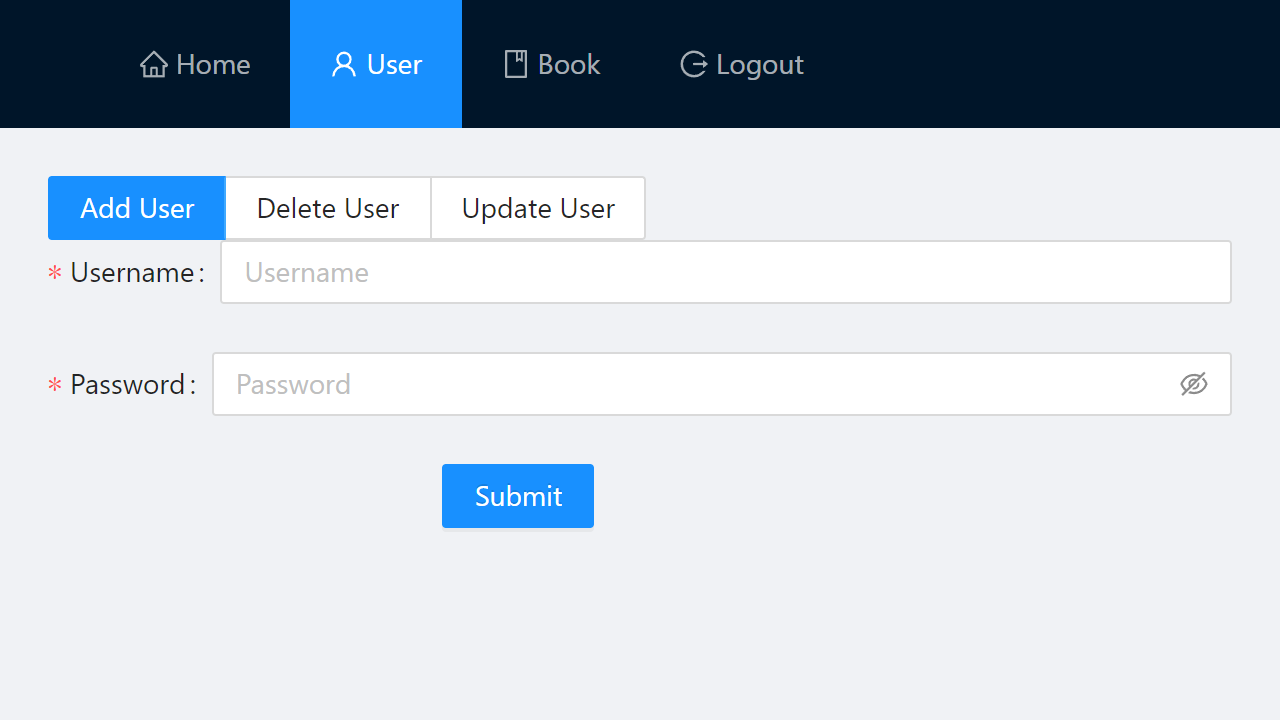
\includegraphics[width=.7\textwidth]{img/front-end/user-add.png}
  \caption{Add User}
\end{figure}

\subparagraph{$\blacksquare$ \texttt{Delete and Update User}}

\texttt{Delete User} and \texttt{Update User} contains more advanced components. When \texttt{Delete User} and \texttt{Update User} are firstly rendered, a request is sent to database to acquire users and their information by using \texttt{useEffect} of React. These pages also utilize pagination and utilities located in the util folder of the user.

\texttt{Delete User} and \texttt{Update User} are pretty similar to each other. Both pages support searching users by both id and username, and the searching option can be changed by using the radio buttons. When an id or username is provided and clicked the search button, a request is sent to the back-end through \texttt{UserService}. When the input area is cleared, the page is updated, and user data is reset. Both pages also support the pagination and pagination setting changes. Admin can change the pagination setting by using the navigation below. When pagination is changed, a new request is sent to the back-end. Additionally, the admin can see the users' information on both pages.

\begin{minipage}{.49\textwidth}
  \begin{figure}[H]
    \centering
    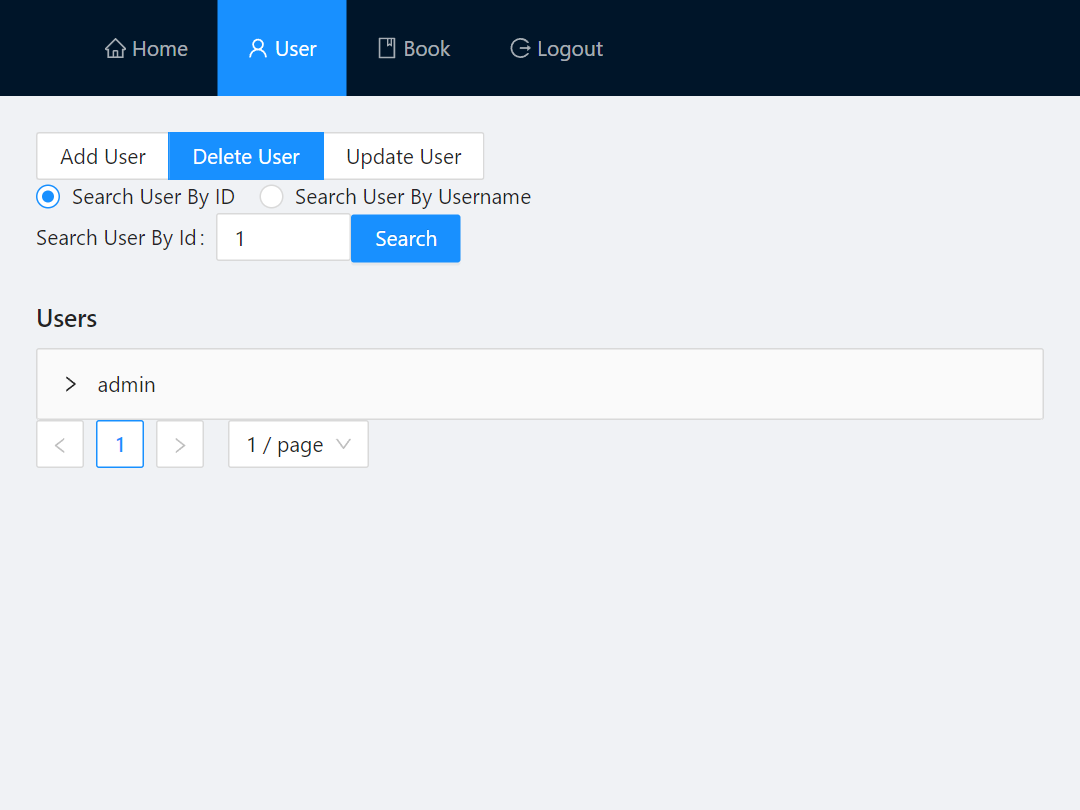
\includegraphics[width=\linewidth]{img/front-end/user-delete-id-search.png}
    \caption{Searching by ID}
  \end{figure}
\end{minipage}
\begin{minipage}{.49\textwidth}
  \begin{figure}[H]
    \centering
    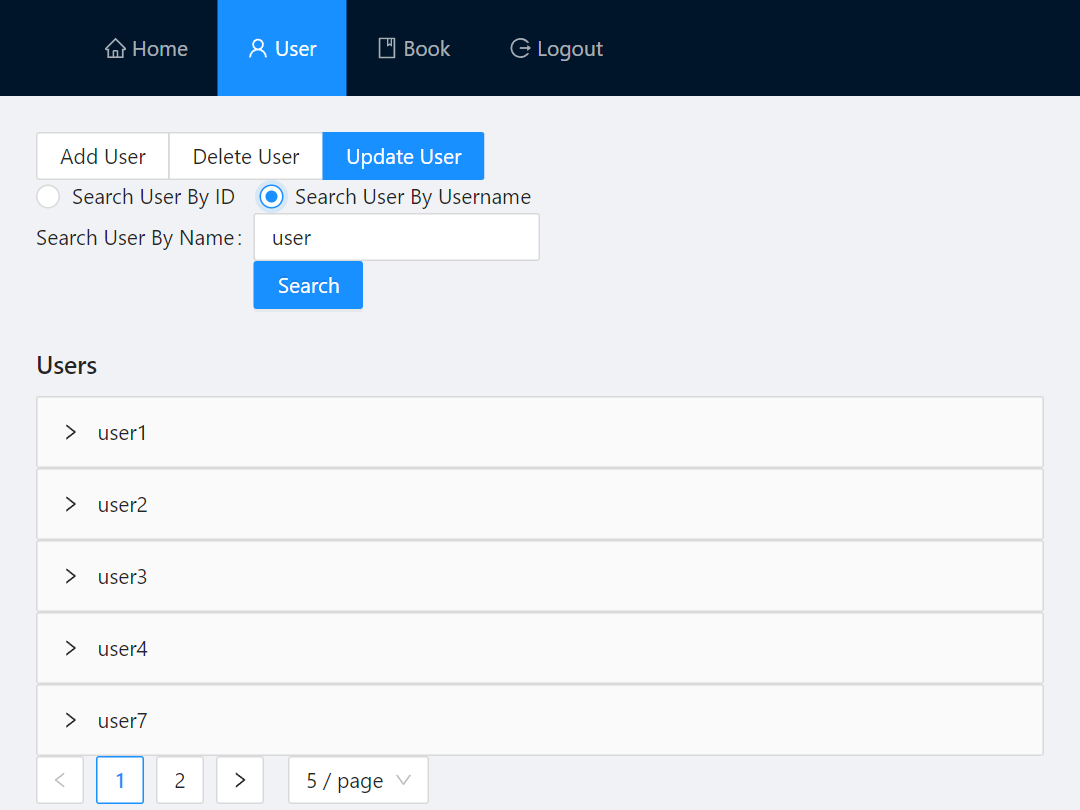
\includegraphics[width=\linewidth]{img/front-end/user-update-name-search.png}
    \caption{Searching by Name}
  \end{figure}
\end{minipage}

Pagination and visualizing the data was the most challenging part for me because there were several aspects I needed to consider. I changed my visualizing method third time for the convenience of development. Because of these changes, I had to change the back-end at some points. This situation causes the loss of so much time for visualizing decisions. However, my job was not done after visualizing the decision because pagination was more challenging than expected. Since I misunderstood some parts and concepts of pagination and its callback functions, I had to spend a couple of hours searching and reading the antd documentation. In the end, I understood what I should do.

The difference between \texttt{Delete User} and \texttt{Update User} is the buttons found in all users. In \texttt{Delete User}, the name of the button is \texttt{Delete User}, and it is used for deleting the user. In \texttt{Update User}, the name of the button is \texttt{Update User}, and when it is clicked password update form appears.

\begin{minipage}{.49\textwidth}
  \begin{figure}[H]
    \centering
    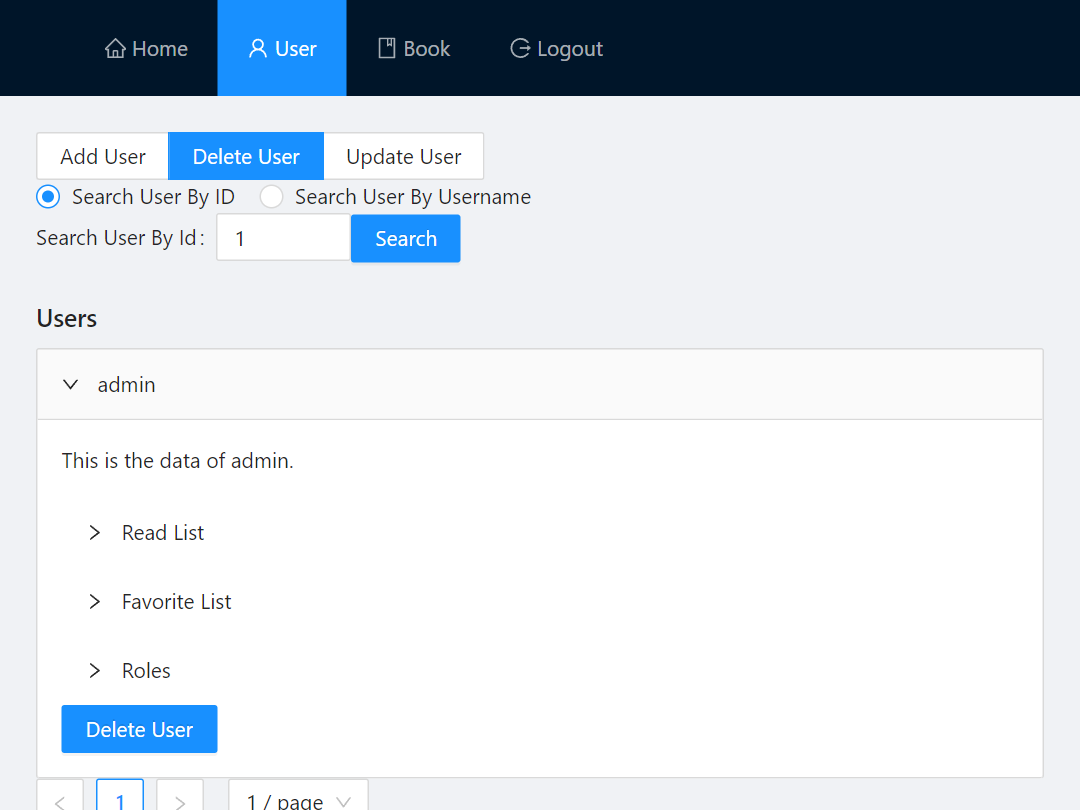
\includegraphics[width=\linewidth]{img/front-end/user-delete.png}
    \caption{Delete User}
  \end{figure}
\end{minipage}
\begin{minipage}{.49\textwidth}
  \begin{figure}[H]
    \centering
    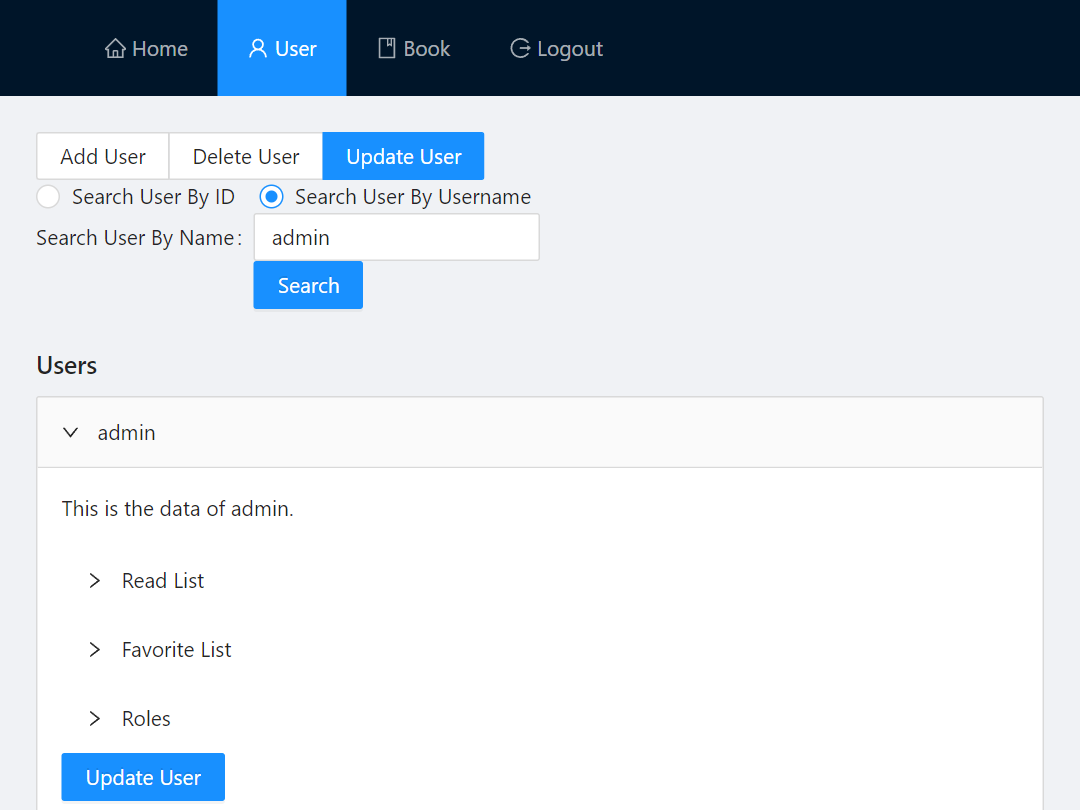
\includegraphics[width=\linewidth]{img/front-end/user-update.png}
    \caption{Update User}
  \end{figure}
\end{minipage}

\paragraph{\texttt{Book}}

When \texttt{Book} is clicked from top navigation, \texttt{Book} page is rendered. On this page, there are three operations: adding, deleting, updating, and listing books. By default \texttt{Book List} is rendered. Although this page is not special, some operations are not allowed to normal users. Therefore, normal users can list books and add/remove these books to/from their lists.

\begin{minipage}{.49\textwidth}
  \begin{figure}[H]
    \centering
    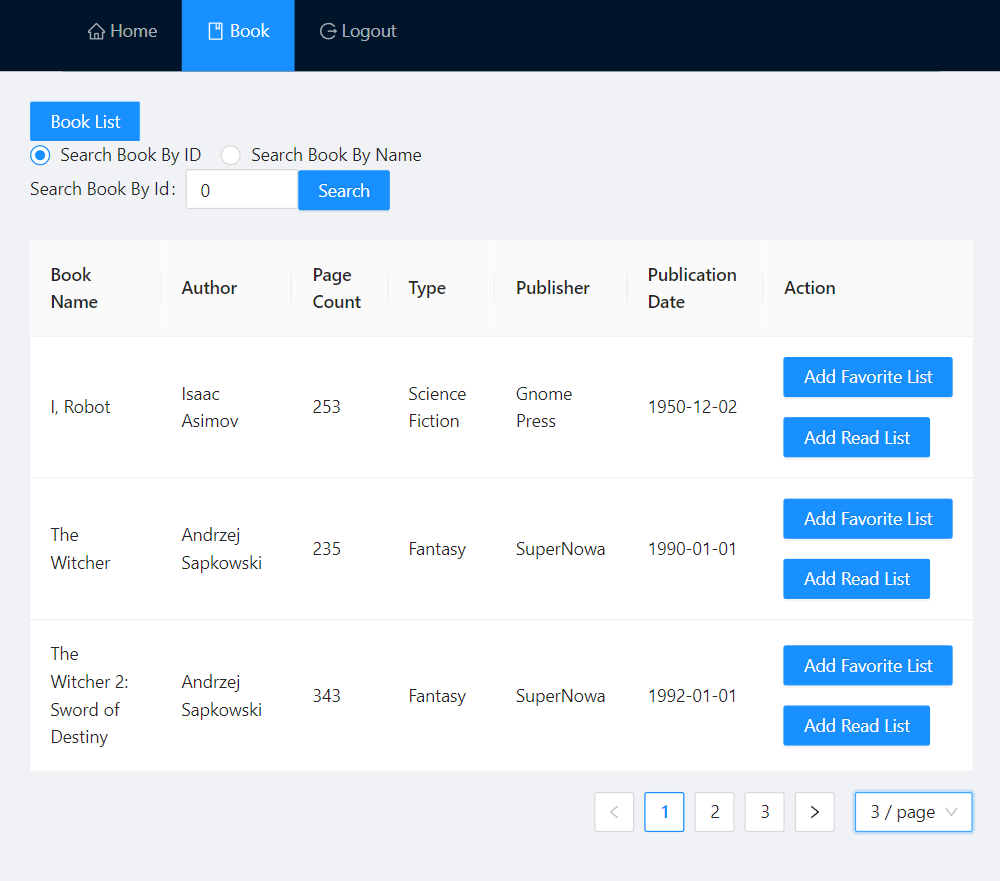
\includegraphics[width=\linewidth]{img/front-end/book-no-admin.png}
    \caption{Book Page for Normal User}
  \end{figure}
\end{minipage}
\begin{minipage}{.49\textwidth}
  \begin{figure}[H]
    \centering
    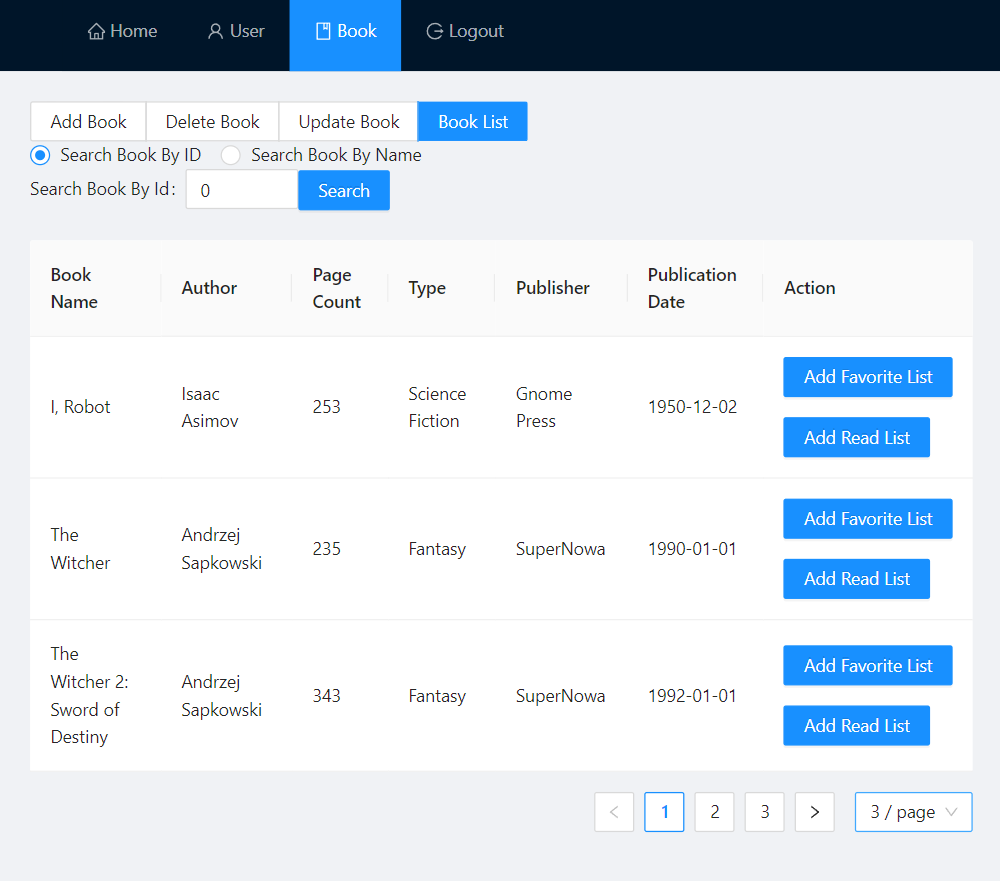
\includegraphics[width=\linewidth]{img/front-end/book-admin.png}
    \caption{Book Page for Admins}
  \end{figure}
\end{minipage}

\subparagraph{$\blacksquare$ \texttt{Add Book}}

This page is for adding a book to the database and is unique to admins. When the option is chosen, \texttt{Add Book} is rendered and provides a form to add a book. The fields of \texttt{Book} entity: name, author, page count, type, publisher, and publication date. All the fields are required, and the date can be chosen from the calendar. When the book is submitted, a request is sent to the back-end with the help of \texttt{BookService}. When the book is saved, the saved book's information is shown below the form. Additionally, the size of the form can be changed by using the `Form Size' radio buttons.

\begin{minipage}{.49\textwidth}
  \begin{figure}[H]
    \centering
    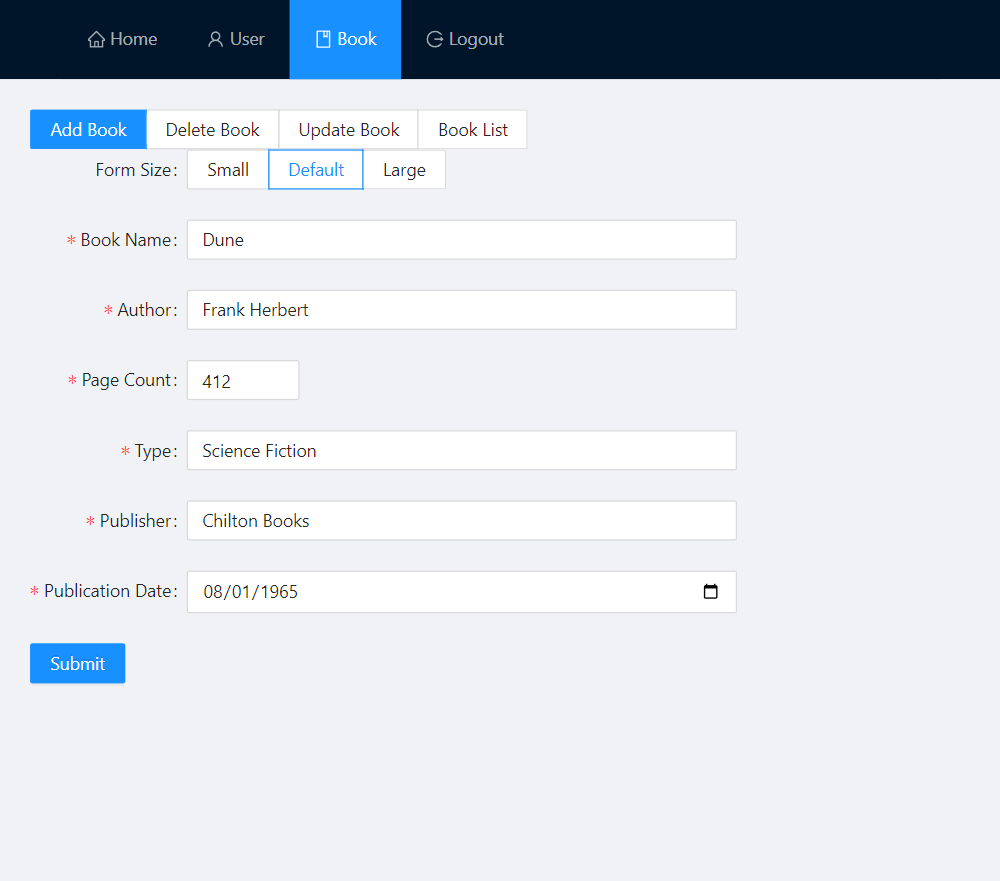
\includegraphics[width=\linewidth]{img/front-end/add-book-form.png}
    \caption{Book Adding Form}
  \end{figure}
\end{minipage}
\begin{minipage}{.49\textwidth}
  \begin{figure}[H]
    \centering
    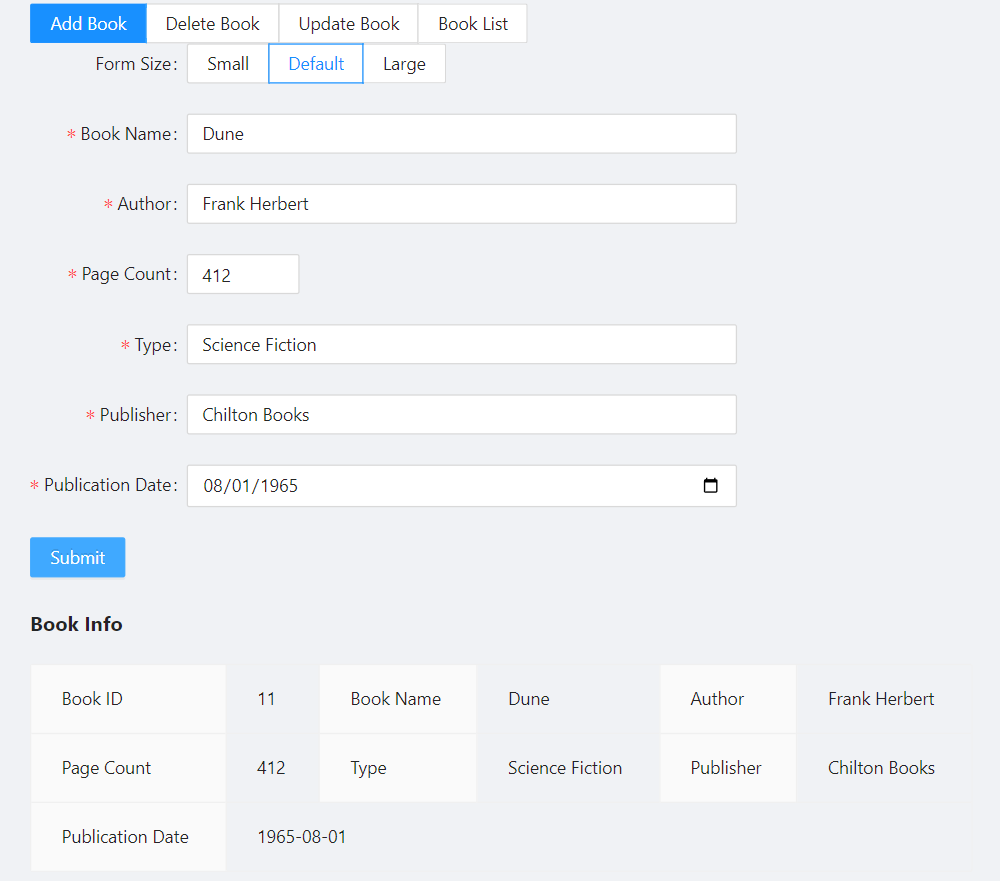
\includegraphics[width=\linewidth]{img/front-end/add-book-added.png}
    \caption{Book Added to Database}
  \end{figure}
\end{minipage}

\subparagraph{$\blacksquare$ \texttt{Delete and Update Book}}

The \texttt{Delete} and \texttt{Update} pages of the book are similar to user's and special to admins. Both pages support searching books by both id and username, and the searching option can be changed by using the radio buttons. Again, when the input area is cleared, the page is updated, and user data is reset. Both pages also support the pagination and pagination setting changes. Admin can change the pagination setting by using the navigation below. Additionally, the admin can see the books' information on both pages.

The only difference between \texttt{Delete Book} and \texttt{Delete User} is the visualizing data. I preferred the `Descriptions' of antd to visualize the data of a book. The differences between \texttt{Update Book} and \texttt{Update User} are the visualizing method and updating form. Only the page count, publisher, or publication date of a book can be updated.

\begin{minipage}{.49\textwidth}
  \begin{figure}[H]
    \centering
    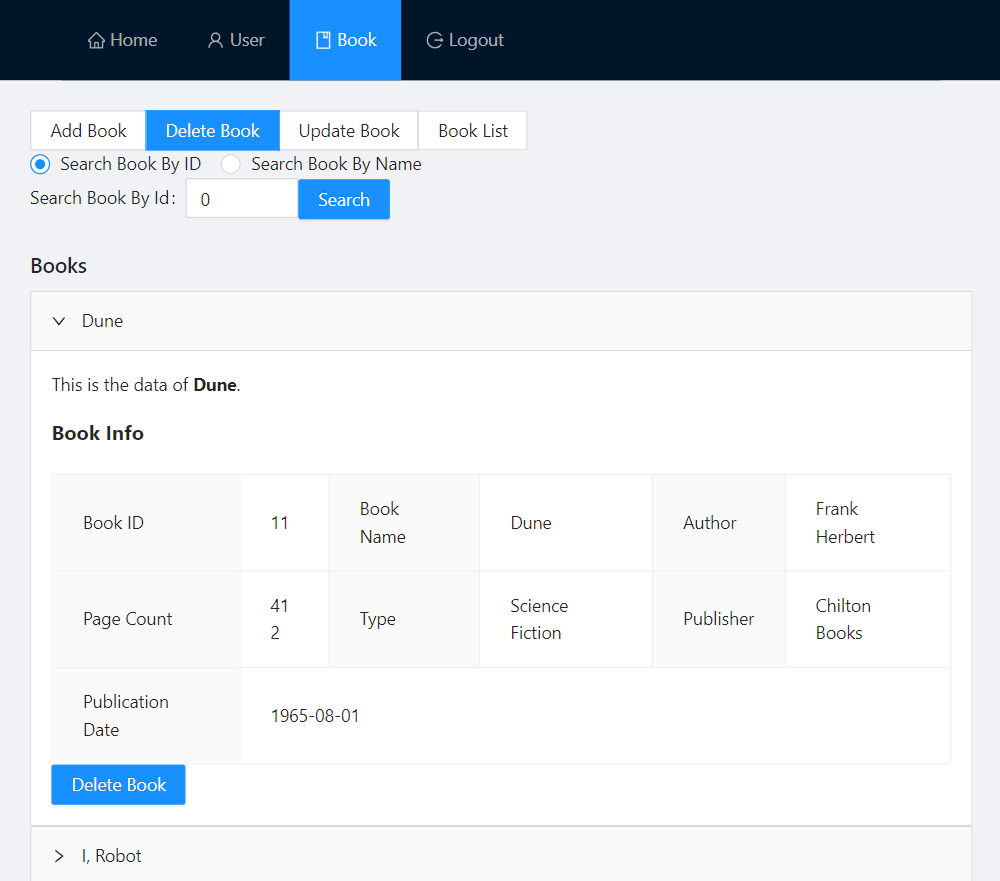
\includegraphics[width=\linewidth]{img/front-end/book-delete.png}
    \caption{Book Delete}
  \end{figure}
\end{minipage}
\begin{minipage}{.49\textwidth}
  \begin{figure}[H]
    \centering
    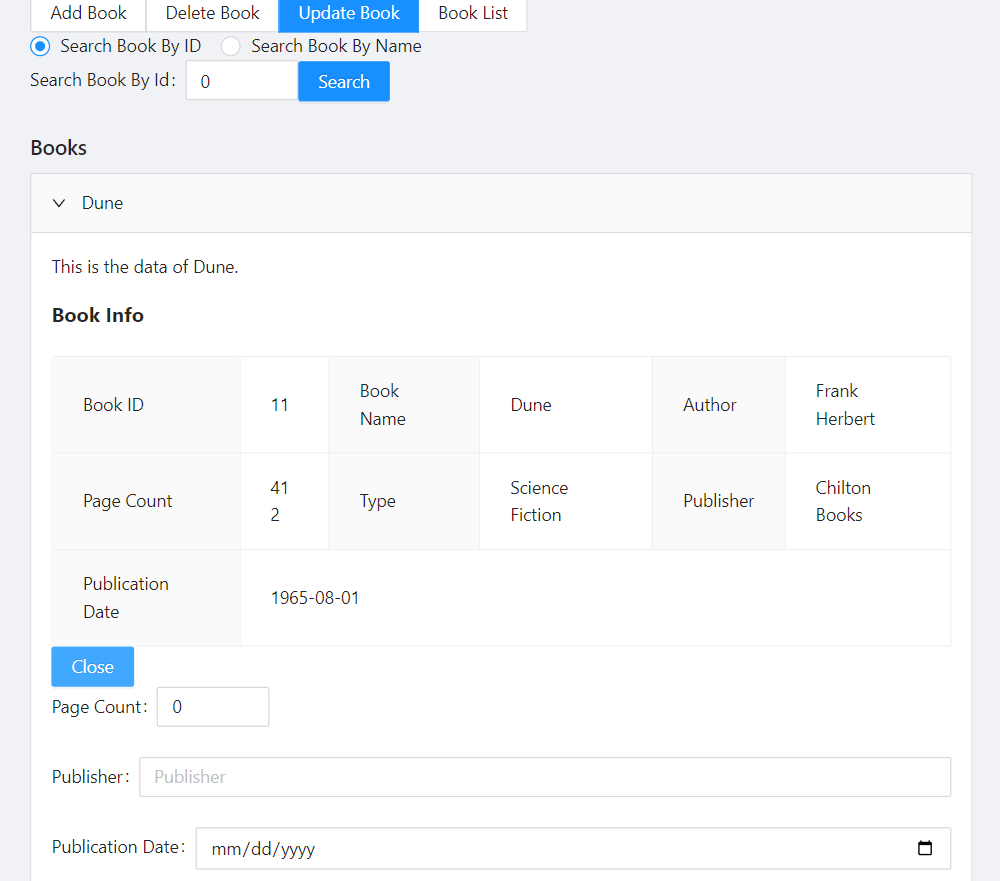
\includegraphics[width=\linewidth]{img/front-end/book-update.png}
    \caption{Book Update}
  \end{figure}
\end{minipage}

\subparagraph{$\blacksquare$ \texttt{Book List}}

This page is accessible by all users and the default rendered page of \texttt{Book} item. `Table' and `Pagination' from antd are used on this page. It lists all the books in the database and provides searching by both id and name. Information about each book is provided in each row, and the actions operate on the book in that row. Users can add or remove the book to/from their read or favorite lists.

\begin{minipage}{.49\textwidth}
  \begin{figure}[H]
    \centering
    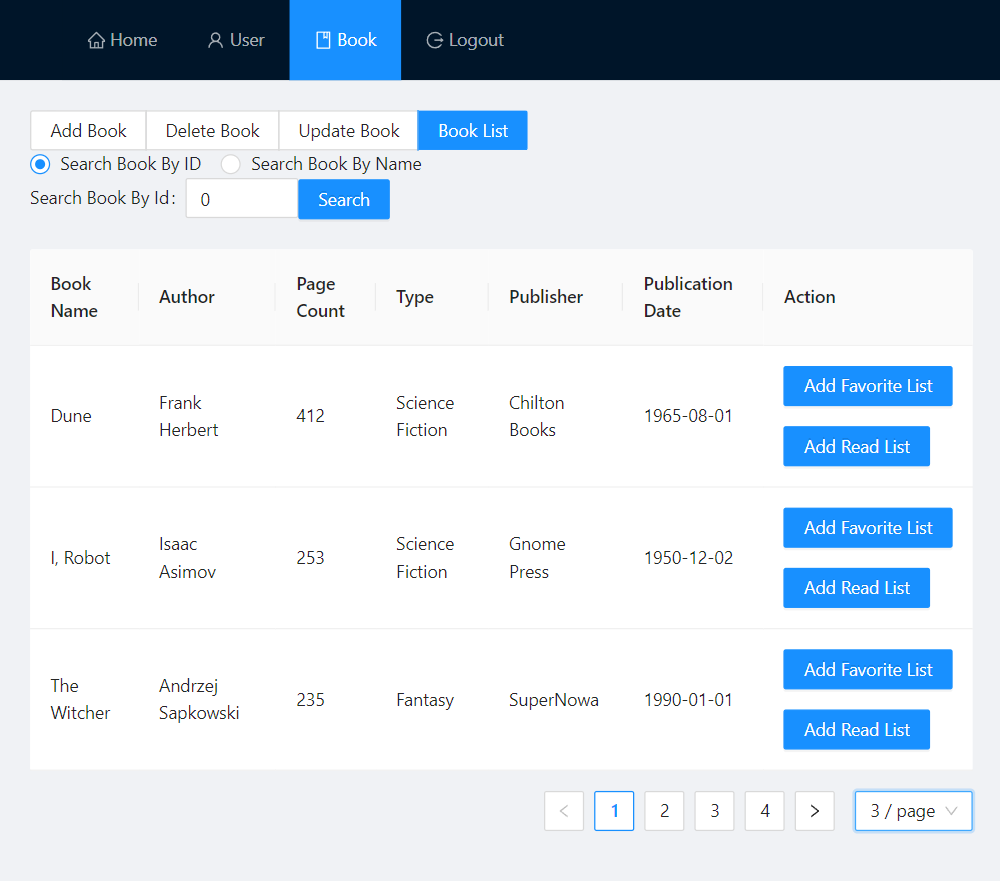
\includegraphics[width=\linewidth]{img/front-end/book-list.png}
    \caption{Book List}
  \end{figure}
\end{minipage}
\begin{minipage}{.49\textwidth}
  \begin{figure}[H]
    \centering
    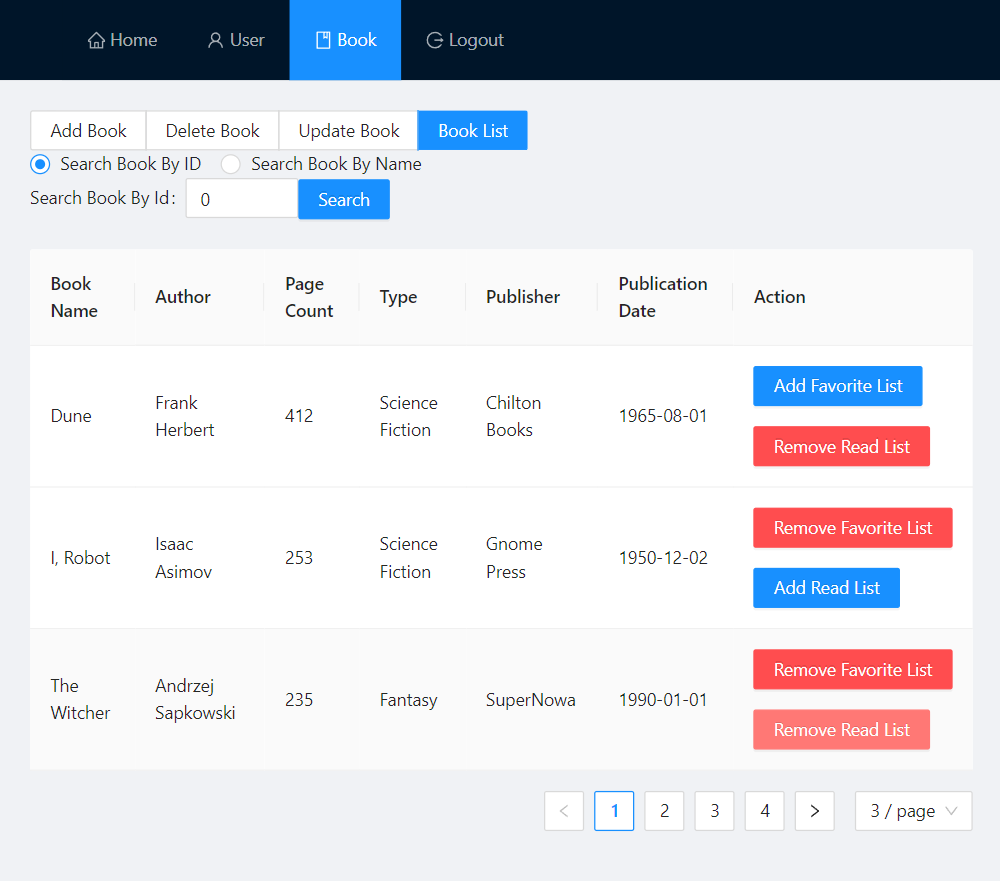
\includegraphics[width=\linewidth]{img/front-end/book-list-example.png}
    \caption{Book List Example}
  \end{figure}
\end{minipage}

If the book is not added to the related list, the action button is blue, and the text of it specifies the adding operation. However, if the book is already added to the corresponding list, the action button is red, and the text of it specifies the removing operation. When the button is clicked, a request is sent to the database, and the book data is updated. As a result, the page is re-rendered with the new state.

This part was hard to code. Putting the action buttons and performing their operations were more complex, aside from the force of the table. It was easy to send a request and save the book to the user's list in the database; however, it was hard to update and re-render the book data and the state of the book. I thought to do this task without getting requests because of the complexity. Also, in the first place, the book information had a problem when the pagination was updated. To solve these problems, I spent several hours.
